\chapter{Transformer Architectures and LLMs}\label{ch_transformers}
\chapterauthor{Jeff Yoshimi, Pierre Beckmann, Tim Meyer}{.5, .4, .1}

% Other general sources
% Helpful annotated python implementation: https://nlp.seas.harvard.edu/2018/04/03/attention.html
% Excellent walkthrough: https://e2eml.school/transformers.html
% Eric T suggests this workshop: https://www.youtube.com/watch?v=quh7z1q7-uc

% There are plans to clarify the definition of generalization, discuss different types of generalization failure (misclassification, high regression error on novel inputs, etc., which then produce many kinds of errors in production AI, from bad translations to mis-pronunciation to misunderstanding queries), and then within these hallucinations as a type (perhaps: LLM outputs that are convincing but factually incorrect).

% Eric S: One striking thing about GPT4 is that you can enter prompts like "Write a four paragraph essay on X" or "First, describe X. Next, describe Y. Finally, describe Z" and it will do it. By the end of the task, the prompt is rather far from the output. It would be nice if this section could explain a bit more how this architecture enables such structured outputs, which one wouldn't expect from say a next-word, next-word, next-word autocomplete on your phone. (GPT3 could also do this, unreliably, so I think the human feedback training isn't essential to this type of task, if I'm recalling correctly that GPT3 was a pure transformer without the human feedback training.)

% Cite Mitchell paper: https://oecs.mit.edu/pub/00hsw4x2/release/1

% Link to Simbrain demo somehow

As discussed in the history section \extref{age_generative_ai}, we have entered a new stage in the history of neural networks, what we are calling the ``age of generative AI'', which should be familiar to you via such tools as ChatGPT. In their most familiar form, a \glossary{large language model} (LLM) based on the \glossary{transformer architecture} generates text responses to text inputs by repeatedly predicting the next word or token in a sequence.\footnote{The concept of token is introduced in chapter \extref{ch_word_embeddings}. Following practice introduced there we will vacillate between ``token'', which is more accurate (since it encompasses punctuation, word parts, and other non-word entities) and ``word'', which is more intuitive.} They are trained on large datasets of everyday text, like text from the internet, which is easily available. As noted in section \extref{age_generative_ai}, it is common to equate ``transformer'' with ``LLM'', but the two concepts are distinct. The transformer is the neural network architecture, while an LLM is just any model of language generation that is based on a large dataset. An LLM can be built out of something besides a transformer, and transformers can be used on things besides language. For example, some state of the art image classification models are now transformer-based, and OpenAI has released an impressive video generation model---Sora, which also runs on a transformer architecture. However, in this chapter we focus on transformer-based models of text generation like GPT.\footnote{There are many other models in this class. As of this writing (June 2024), this includes the open Ai GPT series: GPT, GPT2, GPT3, GPT4, and GPT 4o. It also includes BERT (Google’s first LLM, which is now out-dated), Gemini (Bard), several Claude models (Anthropic;  semi open-source), Llama, LLama2 and LLama3 (Meta), and Alpaca (Stanford; open source). Most of these models can only be accessed online but some can be downloaded and run locally, further fine-tuned, etc. A list of LLMs ranked by how well they chat is here: \url{https://chat.lmsys.org/?leaderboard}.} We will sometimes refer simply to ``LLMs'' by which we mean transformer-based LLMs.\footnote{There are numerous high quality online resources for learning about LLMs. An excellent visual introduction is at this website: \url{https://poloclub.github.io/transformer-explainer/}. Three blue one brown is always excellent on visual intuition and he has a \href{https://www.youtube.com/watch?v=wjZofJX0v4M&list=PLZHQObOWTQDNU6R1_67000Dx_ZCJB-3pi}{\underline{youtube video}}. For a more technical walk through on building an LLM from scratch see \href{https://www.youtube.com/watch?v=kCc8FmEb1nY}{\underline{Karpathy's tutorial}}.}
% GPT as a generic term means “Generative Pre-trained Transformer” (though it is often also used to refer specifically to open AI’s models. Though the transformer architecture can be used in many ways, it became prominent through its use to support large language models (LLMs), which are language models that generate human readable text.}.  Forward ref to pretraining vs fine tuning.

% Discuss topics relating to BERT. (1) Encoders vs. decoders. This terminology likely comes from autoencoders, where we compress data down to a latent space and then decompress it, capturing essential information and then reconstructing it. In the context of transformers, an encoder is responsible for processing input sequences to produce meaningful representations (embeddings), which can be at the word or sentence level (refer back to the word embedding chapter). For example, we can feed a transformer encoder the first halves of hundreds of movie scripts and train it to produce the second halves, or we can train it to predict the first summary paragraph of a Wikipedia article based on the main body of the article. (2) Bidirectional vs. unidirectional is about considering the context in both directions during training. BERT considers the whole context of a token from both the left and right during training while masking specific tokens. This is known as "masked language modeling" (MLM) instead of next-word prediction.\footnote{See \cite{devlin2018bert} for a detailed explanation.} Instead of modeling language as a left-to-right stream of words, where the model predicts the next word based on the previous context (as in GPT), BERT masks a token in the middle of the sentence and predicts it based on the surrounding context. This has advantages over unidirectional left-to-right and concatenated left-to-right and right-to-left models since it creates a truly bidirectional representation where the left and right contexts are joined together. This approach has, however, faced challenges, and for some tasks, left-to-right models like GPT have been found to be more effective. I guess it's still used for some purposes but I'm not sure. Also, I suppose it's not a realistic model of actual production, though perhaps it is a good model of how we represent sentences encoded in memory.
% A relatively clear way to discuss this is as (1) decoder only (GPT, our emphasis), (2) encoder only (BERT), and (3) encoder-decoder (text translation).  // Encoders essentially act like very powerful, context-aware word embeddings—they take an input sequence, process it with self-attention, and produce structured contextual representations that can be used for a variety of tasks. // The core architecture of encoders and decoders in Transformers is nearly identical, with just a few key differences in masking and usage. Of course encoder-decoder has cross-attention

% Add LM vs LLM (and also TLM). On LM see Bender, ``we understand the term language model (LM) to refer to systems which are trained on string prediction tasks: that is, predicting the likelihood of a token (character, word or string) given either its preceding context or (in bidirectional and masked LMs) its surrounding context.''
% So large that Bender et al call it ``unfathomable training data''
% ``We take the term _language model_ to refer to any system trained only on the task of string prediction, whether it operates over characters, words or sentences, and sequentially or not.'' (Bender)

Earlier efforts at text generation and natural language processing used supervised recurrent networks (chapter \extref{ch_supervised_recurrent}), which are, as we saw, in various ways limited. In particular, they can only process a small amount of context, and suffer the vanishing gradient problem. The transformer architecture is basically a complex feed-forward network that can be ``aware'' of multiple kinds of relationships between arbitrarily far-flung parts of an input stream. Because it is a feed-forward network, many of the older techniques covered in this book can be applied to the architecture. In particular, all the lessons of the deep learning revolution (section \extref{deep_revolution}) apply here, and indeed, transformers are many-layered deep networks (chapter \extref{ch_cnn}) that make good use of both \glossary{representational width} and \glossary{representational depth}. They can be trained on large datasets using highly optimized parallel hardware. Like all the other networks discussed in this book, they are not just useful as engineered tools, but are highly relevant both to neuroscience and cognitive science, and seem to develop meaningful internal representations. 

We start with preliminary discussion of how transformer-based LLMs are trained using highly available text data, and how a special recursive trick can be used to make a feed-forward network that only predicts next words still produce meaningful conversational outputs. We then discuss how the transformer architecture itself works. Finally we consider how LLMs are utilized and evaluated and the relevance of these models to cognitive science, neuroscience and other areas.

Changes in this area are rapid, and the relevance of these areas to cognitive science is only now being studied, so updates to this chapter are expected.

\section{Learning to speak Internetese}

In section \extref{languageModelsRecurrent}, we saw how recurrent neural networks trained on example text can learn to speak in a way that reflects the statistical properties of the training data. A network trained on Shakespeare will start to speak fake Shakespeare, a network trained on real math can generate fake math, etc. Large language models using transformers do the same thing, they just do it much better. The architecture is better suited to the task, as we will see, and they can use much larger datasets (hence ``large'' being added in front of ``language model''). In fact, the training set for GPT-3 was not all of Shakespeare, or just a bunch of math papers, but rather a large subset of the \emph{entire internet}, which included all of Wikipedia, a few compilations of books, and a web-scraped archive of the internet called ``common crawl'' (\url{https://en.wikipedia.org/wiki/Common_Crawl}). See figure \ref{gptDatasets}. Similar datasets continue to be used on LLMs, so if you've ever written anything online, there is a decent chance it is part of the training data for one of these models. 

Since all of Shakespeare is on the internet, and discussions of every topic of human endeavor from physics to history, and plenty of gossip and randomness about popular culture and everything else, these models can talk about all of these things. They can statistically generalize from their training data, which consists of a large part of the internet, which in turn encompasses many of the books and recorded knowledge of human history. In a sense, these models learn to speak ``internetese''. 

\begin{figure}[h]
\centering
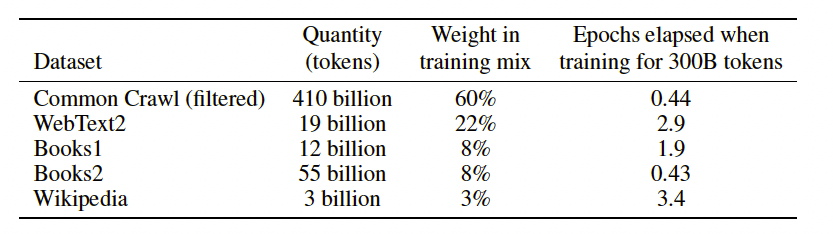
\includegraphics[scale=.4]{./images/gptDatasets}
\caption[From \cite{brown2020language}.]{The datasets used to train GPT-3. The data mostly consists of data scraped from the internet, but lots of books and all of Wikipedia are also included.}
\label{gptDatasets}
\end{figure}

% Add more recent sources on the Turing Test claim. There are already as of 2025 multiple papers on the topic.
% Turing test passed now? (Bergen): https://arxiv.org/abs/2503.23674
The results are impressive. The texts these models produce are no longer obviously fake in the way the examples from section \extref{languageModelsRecurrent} were. In fact, in some cases they arguably pass the \glossary{Turing Test}, a long-standing test for artificial general intelligence, answering questions and producing convincing  text in response to prompts. Whether LLMs really pass the test is a matter of ongoing controversy. This is discussed further in section \ref{llmPhilosophy}.

\section{Training Using Next-Word Prediction}

Recall from chapter \extref{ch_data_science} that a labeled dataset consists of inputs and targets. As noted there, this kind of labeled data can be hard to obtain. We might have lots of pictures of people but not know the names or identities of the people in the pictures, or lots of pictures of cats and dogs but not whether a given picture is of a cat or dog. Creating targets for a large dataset is labor-intensive, requiring humans to manually label each picture.

% Eric T: Maybe mention this is also called self-supervised learning because it doesn’t require labeled data.
% Need a bit more fanfare on the embedding step, since it is the first step in the pipeline, but not sure the best way to integrate it into the discussion
% Add glossary item for auto-regression
% Tim feedback: currently the discussion makes it sound like a random sequence is extracted from a training text. However we window across and then use the "Christmas tree" method. This needs to be made clear. An image could be used to clarify. In the UC Merced quote can draw a window of length context size and then show several steps of it moving. Perhaps link to a page showing the full set of training samples and a few parameters what the full number would be, and say the formula for how many samples we'd get.
LLMs like GPT use a special method (sometimes known as auto-regression) to take \emph{any passage of text} and convert it into a labeled data set that can be used to train a neural network. The trick is, roughly, to treat a sequence of text tokens (minus the last token in the sequence) as an input, and to treat the final token in the sequence as a target. More specifically we use vector embeddings of the tokens as inputs and targets. The great thing about this method is that it can be used to generate a labeled dataset from any text document. No longer do we have this difficulty of finding labeled data. Just take any old piece of written text, and you've already got multiple training examples, just by taking concatenated vector embeddings of different sequences of tokens as input and vector embeddings of the next tokens after those sequences as targets.

For example, consider this block of text adapted from the Wikipedia page for UC Merced:

\begin{quote}
The University of California, Merced is a public land-grant research university in Merced, California. It is one of the ten campuses in the University of California (UC) system. Established in 2005, Merced is the newest campus within the UC system.
\end{quote}

From this, we can create a bunch of training examples, a list of input / target pairs. We might use ``The University of" as an input, and then ``California'' as a target. We simply associate each token in the input with a vector using a word embedding (chapter \extref{ch_word_embeddings}). The target is also vector encoded, but in a different way: as a one-hot encoding over all possible tokens, where all entries in the vector are 0 except the actual next token (we discuss this further in section \ref{llmOutput}). In this way we can build a table of input-target vector pairs, which we can use to train a feed-forward neural network. For a sense of the idea, see figure \ref{nextWordPrediction}.\footnote{Note that normally a word like ``University'' would be split into multiple tokens, but we are keeping things simple here. Some information on tokenizers is in chapter \extref{ch_word_embeddings}.} 

\begin{figure}[h]
\centering
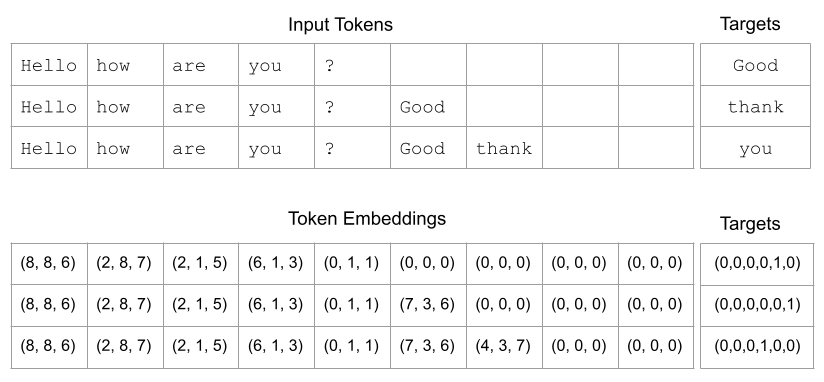
\includegraphics[scale=.45]{./images/contextWindow.png}
\caption[Jeff Yoshimi]{How text sequences can be converted into training datasets using the method of auto-regression. A set of tokens is converted into vectors using a token embedding (the vectors shown are arbitrary, just to illustrate the idea), and by concatenating these vectors we get an input vector. The next token in the sequence is encoded as a target using a one-hot encoding over all tokens (in this case there are seven tokens: six words and the question mark)}
\label{nextWordPrediction}
\end{figure}

Note that the word embedding in this example is 4-dimensional (each token is associated with an array of 4 numbers, a vector in a 4d space). In real LLMs, this ``embedding dimension'' is quite large, for example over 12,000 for GPT-3 (see figure \ref{gptParams}). 

In practice, a sequence of tokens is converted into a matrix where each row corresponds to the token embedding for one token. This matrix is the actual input to the neural network. So unlike earlier, simpler neural networks, which transformed vectors to vectors via weight matrices, here we are transforming \emph{stacks} of vectors by matrices. \footnote{What is actually fed to the transformer is a batch of these token embedding matrixes, that is a rank-3 tensor (see section \extref{sect_tensors}).}  Figure \ref{nextWordPrediction} illustrates the idea, and introduces some useful terminology. Notice the ``you'' occurs twice in the stack, and is associated with the same row vector.

\begin{figure}[h]
\centering
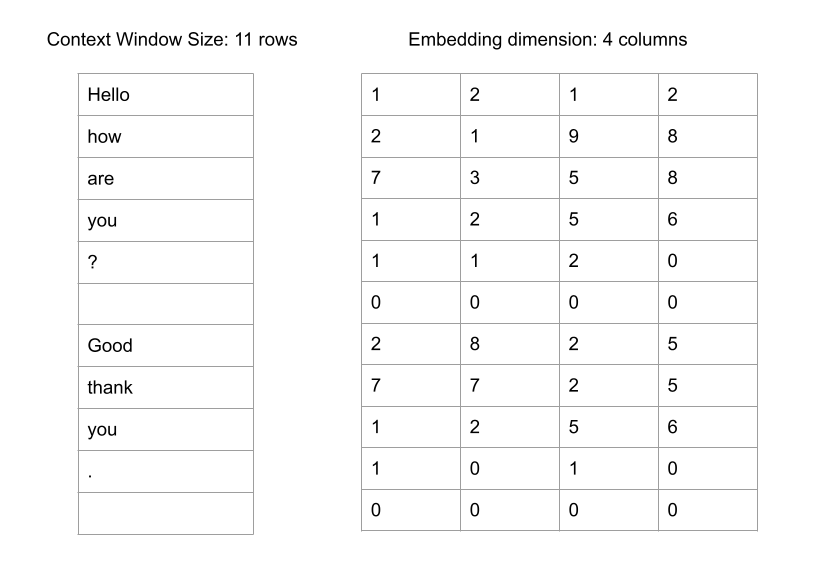
\includegraphics[scale=.45]{./images/contextWindowAsStack.png}
\caption[Jeff Yoshimi]{The context window is associated with a matrix that can be thought of as a stack of vectors, one for each token. }
\label{nextWordPrediction}
\end{figure}

There is a key conceptual model that occurs here that is useful to fix in mind, since it's key to understanding LLMs. We can think about the context window as a stack of tokens converted into a stack of vectors, where the vectors correspond to embeddings of the tokens in a vector space that then get transformed as they travel through the network. Thus the repeated ``you'' will change its representation as it is processed. This may seem confusing at first; don't the numbers get all jumbled up when we matrix multiply? But note, as we saw in the linear algebra chapter (chapter \ref{ch_linear_algebra}), a stack of $N$ row vectors multiplied by a matrix produces another stack of $N$ row vectors. Each row is \emph{separately processed} by the matrix. As a result, we can track the transformations a token's representation goes through as it makes its way through a network.\footnote{This idea is illustrated in section \extref{wordEmbeddingMatrix}, where it was described as a ``token embedding matrix''.}
% Millier calls this a "residual stream".
% The "linear map hypothesis"
% Vector embedding and tracking one vector as it's transformed through the layers.  3b1b does a lot of this.  Integrates well with earlier chapters and integrates well with the new simbrain pictures.

% Tim feedback: positional feedback happens too fast.  A mystery is thrown at the reader. Take time and unpack. To make it clear concretely what happens, see the picture I made (positionalEncoding.png). Clarify position is position in sequence.  But it's also confusing how this doesn't mess up the semantics of say king - queen  = man - woman.  The response is something like we now have slightly enriched semantics, like king-at-start-of-sequence, etc., and noting that gradient descent will discover the same things it did before, PLUS representations that are sensitive to position. Separate question: why aren't the weights enough to provide positional encodings, since there is some implicit ordering in it. 
% Another option for positional encoding is to just leave it out from the discussion
One interesting feature of transformers is that the processing they do does not inherently care or know about the order of tokens in a sequence. Thus, the tokens in a token embedding matrix are in a sense unordered (their position in a stack is an order, but this information is not easily available to the network given how it processes information), which allows for super-fast parallel processing. Thus a \glossary{positional encoding} is used to modify the vectors in a token embedding matrix, often by using a trigonometric function (like sine or cosine) that simply adds more or less to the numbers in the vectors depending on where they are in a sequence.\footnote{This is a kind of feature engineering trick; see chapter \extref{ch_data_science}.}  In figure \ref{transformerBlockSimple} the encoding subtracts 1 from each component of the word embedding for ``Hello'' (which was $(8,8,6,1)$ for the sample embedding in figure \ref{nextWordPrediction}).
  
\section{How Text is Generated from a Feed-Forward Network}

% Pictures needed for recursion trick and context window. E.g take second figure in this chapter and add some arrows or numbers showing how to generate sequences.
% Clarify somewehere that padding is not usually used at the end of a context window. The stacks of vectors and self-attention matrix can be variable-sized depending on the length of the current chat. This is missing.

One confusing thing about figure \ref{nextWordPrediction} is that we go from a large input covering a whole set of tokens to a single token as output. So great, we can predict single words. But how do we go from single words to generating long text outputs, or having conversations? In fact, in hearing about generative AI as ``next word prediction'' machines, you may have sometimes wondered how such complicated things can happen when all they models do is predict next words.

% More discussion of special tokens like end-of-sequence is probably needed, and maybe further up.
The answer is by using what we can call the ``recursion trick''. This trick allows us to take a feed-forward network that only predicts next words and use it to produce streams of text output. In fact, it's remarkably simple. We feed a network a set of inputs corresponding to string of text, and it produces an output corresponding to the predicted next token. That output is then appended to the previous input, and this longer input is now fed back to the network. This process is repeated to produce a stream of text outputs. This technique can be used to generate unending sequences of text from any prompt.\footnote{Notice that this is a kind of recurrence, and arguably this makes LLMs used in this way a kind of recurrent network. Outputs are fed back in as part of inputs. However, the outputs are text that must be converted back to text inputs, which are then vector encoded. In fact, recurrent networks were originally used for text processing, as we saw in chapter \extref{ch_supervised_recurrent}, but it turns out that fancy feedforward networks used in this way outperform them. (In those cases, a vector representation of each token in the sequence would be presented separately: ``hello'', ``how'', ``are'', ``you'', and ``?'').} The prompt is our input, and then answers are generated using the recursion trick. Text will continue to be generated until a special end-of-sequence token is reached.\footnote{An important step forward with ChatGPT was its ability to mimic human conversation or ``chat''. This was achieved using specialized training techniques, particularly Reinforcement Learning from Human Feedback (RLHF). RLHF uses reinforcement learning with human input--such as when ChatGPT asks users to rank responses--to refine its conversational abilities.  This human feedback is used to develop a reward model that is used to update the network’s parameters, incentivizing it to produce a more human-like cadence of responses.} 
% Promote this note.
% The when-to-shut-up circuit. Humans have to learn this too, so it's anther example of an engineering necessity motivating an interesting psychological question
% Get details of how the stop tokens (name?) work. They are there already presumably. But this counts as fine-tuning since it's a way to make them occur at more appropriate times.

So this gets us one response. But then you type a new question. That \emph{entire question} is appended to the \emph{entire past conversation} including both what you and GPT have said so far. 

Suppose, for example, we want to ask a network ``hello how are you?'' The input to the network is the whole sentence $\{$``hello'', ``how'', ``are'', ``you'', ``?''$\}$. Let's  not worry about the vector embeddings, and just see the general idea, as shown in figure \ref{gptRecursedInputs}. Notice that the initial prompt is the initial input, but then the prompt \emph{and} the first word of the response are used as the next input, and this process can be repeated until a response is written out.
  
\begin{figure}[h]
\centering
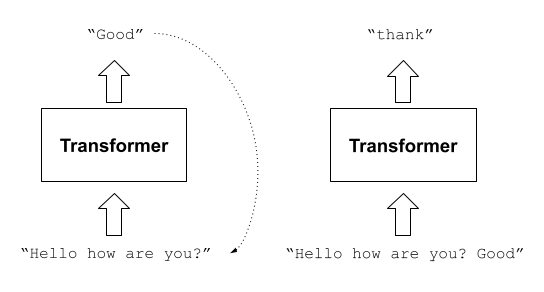
\includegraphics[scale=.7]{./images/gptRecursedInputs.png}
\caption[Jeff Yoshimi]{A schematic view of how ``conversations'' are generated from a feed-forward network in systems like GPT. The output from one moment is added to the end of the input, and the new input is then fed in. The process is repeated to generate a full response.}
\label{gptRecursedInputs}
\end{figure}

Of course, as we keep doing this, the inputs to the network get larger and larger, and there must be some limit to how far we can go, right? The answer is yes. Any LLM specifies a fixed-length \glossary{context window}. At the start of a session, this window is mostly zeros, except for the initial prompt. In a dialog, the prompts from a person and the responses from the LLM are both included until the context window is filled. Thus, if the context window is large enough, whole series of back and forth conversations can be processed. All the prompts and responses up until the current point are part of the input, and then the LLM uses the recursion trick to generate new responses that are sensitive to everything that's been discussed thus far. When the system runs out of slots in its context window, items are simply removed from the start of the context window (from a computer science standpoint, this is a queue). This is intuitive in figures \ref{nextWordPrediction} and \ref{gptRecursedInputs}. These context windows can be remarkably large. GPT-3 has a context window of about 2000 tokens or about 6 pages of text, and early versions of GPT-4 had context windows of 32,000 tokens or about 72 pages of text. 

Here is the idea in more detail, in a way that begins to give a sense of how some of the details work, for a highly simplified example. The outputs are softmax, discussed below (section \ref{llmOutput} and in chapter \ref{ch_act_functions}), with one node for each token in a very small vocabulary. The network takes the stack of token embeddings as input and produces a probability distribution over these tokens as output.  See figure \ref{transformerOverview}.

\begin{figure}[h]
\centering
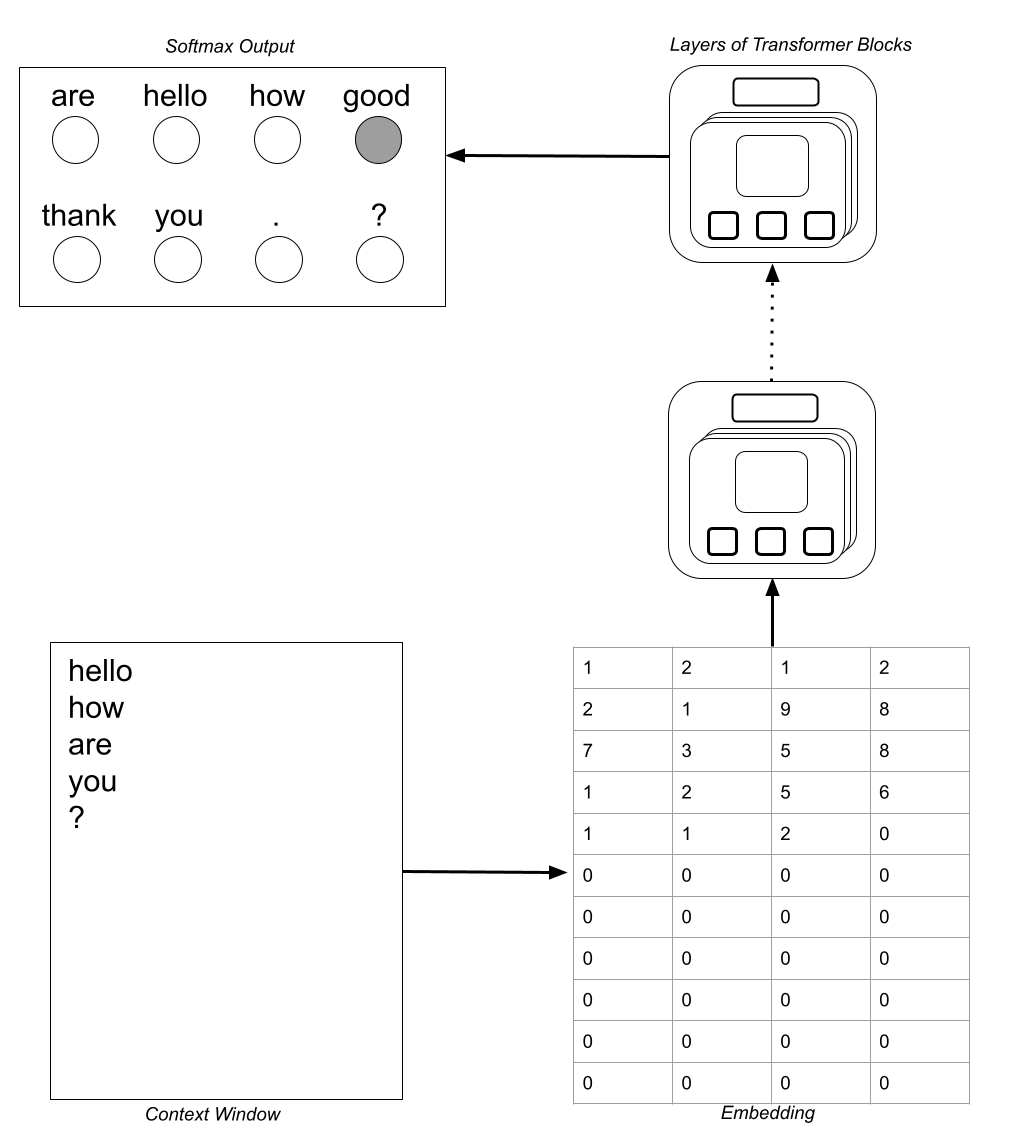
\includegraphics[scale=.2]{./images/TransformerOverview.png} \; \; \; 
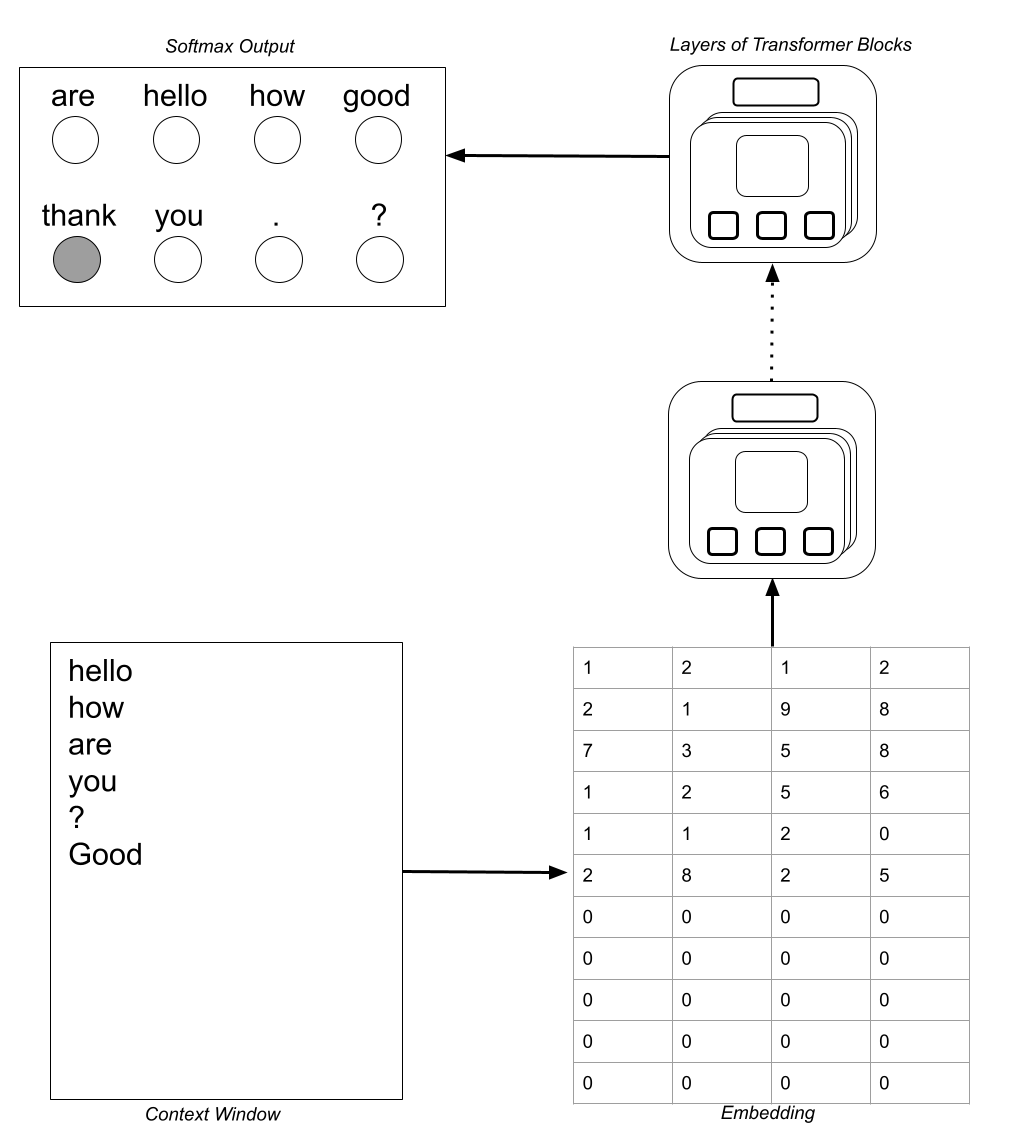
\includegraphics[scale=.2]{./images/TransformerOverview2.png}
\caption[Jeff Yoshimi]{A first look at the entire process of a conversation unfolding through a network, showing the stack of word embeddings associated with the context window, the transformer blocks, and the softmax output. Note that the most active output is associated with a token that is added to the context window on the next time step. Shown are two time steps. On the left the network has output a response of ``Good'' in response to the query, and that output is placed in the context window using the recursion trick.}
\label{transformerOverview}
\end{figure}

\section{The Transformer Architecture}\label{transformers}

We have thus far covered high-level features of how LLMs work, but have treated the transformer as a black box. The time has come to open the box. How does the fancy feed-forward network at the heart of these models work? Its power rests on a few novel architectural innovations, which combine representational width and representational depth with a special form of context awareness. All the things we've seen about other neural networks apply here. It is a kind of deep feed-forward network, which uses a huge amount of training data. But the key innovation is that within each ``layer'' it can develop many forms of context representation, which relate all the tokens in a context window to each other.

\subsection{Blocks}

% A big pass is coming esp. here. One thing to possibly do is to show the embedded tokens stacked in matrix form so it's clear the embedding is done with matrix operations. This also needs to  be cohered with the NLP chapter.

% On KQV. 
% Broadly we can just think of KQ as a representation that facilitates token-to-token context. That is the big picture.
% we need two things to make a context representation, and then we need a third thing to push through it
% For K and Q, see https://e2eml.school/transformers.html which makes clear how the key is like a lookup (but need to work on this). Queries and keys both correspond to tokens. The queries are source terms, the keys target terms.  The key scans across the past-tokens (triangular mask) and selects information useful for predicting.  This also links to the query based attention stuff from McLelland.
% For  V, see Tom Yeh (https://www.byhand.ai/p/8-can-you-calculate-a-transformer), he focuses on the attention matrix and the "attention weighted features" (for us v times the attention matrix). From that perspective V is just a kind of reshaping of the input features into a form usable by the transformer  

% Eric T comment: The canonical type of example to use, that I think would be helpful, for why we are taking these dot products of influence across tokens, is a standard disambiguation example (e.g., `I went to the bank to cash my paycheck`, vs `We ate a picnic on the bank`). The transformer lets you come up with a new embedding that better represents the semantics of the tokens based on their context. The meaning of ‘bank’ just based on the original token embedding (say, from word2vec) is unclear but the self-attention step will allow meanings to propagate across tokens and push them in the right direction.   This point about context is in your chapter, but I worry it is getting lost a bit in all the technical details, so I think it  may deserve a bit more focus about how it's supposed to work. You can make this point even without mentioning key/value/query stuff or multiple heads (multiple heads is sort of a secondary or even tertiary point). The K/V/Q matrices add to this contextualization the power of tunable parameters (this is my admittedly limited understanding based partly on this really good video: https://www.youtube.com/watch?v=tIvKXrEDMhk ).

% Eric S below: "Compares" is vague. How to give a sense of it right up front
The transformer architecture \cite{vaswani2017attention} contains layers or ``blocks'', which are specialized to process the large context windows that are fed to the network as input. With training, they learn to find long-range dependencies between different parts of a context window. Recall that the context window  includes an original prompt, its own response to that prompt, etc.; it includes the \emph{entire exchange} you've had with GPT up to the current point, so long as it fits in the context window. Each block combines a ``self-attention'' layer with a traditional linear layer and several other mechanisms (see figure \ref{transformerBlockSimple}). The self-attention layer is where the magic happens. One part of this layer compares each token in the context window to every other token in the window. In our simple example, ``hello'' is compared to ``how'', ``are'',  ``you'', and also to itself. These comparisons are used to create a representation of the sentence that reflects dependencies between the words. All words are compared to each other in the context window, so that no matter how far apart they are, they can still influence each other. The self-attention mechanism learns what relations between words in a context window are important; in a sense it learns what to focus on (hence ``self attention''). This ability to find meaningful relationships within an input sequence is part of why transformers are relevant to cognitive science, as we will see.

% Cohere this with the new images
\begin{figure}[h]
\centering
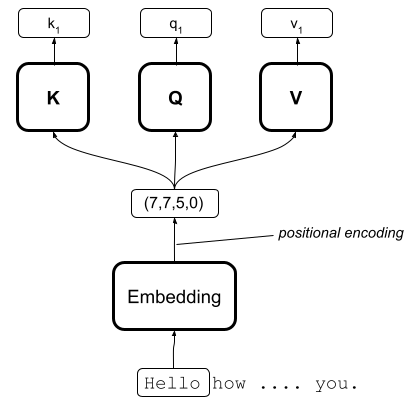
\includegraphics[scale=.4]{./images/transformerBlockBasic.png}
\caption[Jeff Yoshimi with consultation from Tim Meyer.]{Part of a transformer block. Each token in the context window is converted into a vector using the word embedding, then transformed using the positional encoding. This vector is then multiplied by three matrices $\textbf{K}$, $\textbf{Q}$, and $\textbf{V}$ to produce three vectors. These operations can be done concurrently and can thus run on fast parallel computing hardware. The resulting vectors will be used to produce a representation that captures relationships between items in the context window. Bolded items are matrices that are updated using gradient descent.}
\label{transformerBlockSimple}
\end{figure}
% The positional encoding does not fit the graphical conventions. There is no arrow, and it's not clear from the diagram what it does. Work with Tim on improvements.  Should it be its own block?
% More on normalizing. See neuralnets.txt. Also need a picture to show that input and output are same-sized.

The details of what occurs in a block are not developed in detail here though we are planning to expand the discussion in future versions of this chapter. Here is a rough sketch of what happens. Each input token in a context window is first converted into a vector using a vector embedding (chapter \extref{ch_word_embeddings}). (In practice, all of the operations described here are performed on batches, or ``stacks of vectors'', rather than single vectors, but we focus on single vectors to make things simpler). This vector is then simultaneously matrix multiplied by three weight matrices labeled $\textbf{K}$, $\textbf{Q}$, and $\textbf{V}$ to produce three vectors: the key, query, and value vectors. This is what is shown in figure \ref{transformerBlockSimple}. Note that the matrices, in bold, are part of what is trained in this architecture.
% Bold is trained, non-bold is computed. Include Simbrain screenshot? 
% Also clarify that all the computations happen on batches

% More on normalization, "scaled dot product"
The key and query vectors are then multiplied (using a dot product) in all possible combinations and then normalized to produce a context representation. This is shown in figure \ref{selfAttention}. These are also called self-attention scores. These scores capture relationships between tokens in a context window. The value vectors (not shown in figure \ref{selfAttention}) are then matrix multiplied by the self-attention matrix to produce outputs that are further processed by linear layers internal to the block.

\begin{figure}[h]
\centering
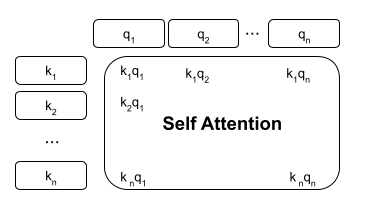
\includegraphics[scale=.6]{./images/selfAttention.png}
\caption[Jeff Yoshimi with consultation from Tim Meyer.]{Scaled self attention matrix generated by multiplying key and query vectors (using the dot product). Value vectors (not shown) are then multiplied by this matrix to produce the output of one head of a block.}
\label{selfAttention}
\end{figure}

% Eric S: At multiple heads: Can you explain a bit more in ordinary language what the functional importance of these transformation is?  Maybe some examples would help. What kinds of things generate high vs low self-attention?
Within each attention block, there are multiple attention ``heads''. Each head carries out all the operations described above: it projects the input from the previous layer (or the embedding in the first layer) into separate spaces through unique projection matrices for $\textbf{K}$, $\textbf{Q}$, and $\textbf{V}$. These projections result in smaller vectors for each head.\footnote{The dimensionality of each head is often the embedding dimension divided by the number of heads, so that when the outputs are concatenated, the original dimension is restored. In figure \ref{gptParams}, the number of inputs to each head, $d_\text{head}$, is equal or almost equal to the embedding dimension $d_\text{model}$ divided by the number of heads $n_\text{heads}$.} For example, if the embedding dimension were 9, it might be projected into three separate 3-dimensional heads.\footnote{Thus, for each head, the $\textbf{K}$, $\textbf{Q}$, and $\textbf{V}$ matrices would typically have dimensions $3 \times 9$, where 9 corresponds to the input dimension from the previous layer, and 3 refers to the reduced dimensionality for each head (note that for efficiency, these matrices are often combined into a single larger matrix.)}

% Mention slicing as a way of extracting a subset of elements from an array, matrix, or tensor.
% The query asks a kind of question, and the key is a kind of answer. See 3b1b. 

As a result of this multi-head attention, the network can learn \emph{multiple} ways to compare words in the sentence to each other, a bit like how a convolutional network (section \extref{convolutionalLayer}) develops \emph{multiple} filters to analyze an image, what we have also called representational width. The results of these different attention heads are combined and as a result each layer of a transformer network involves a sophisticated representation of the sentence that represents multiple types of inter-word dependency. 

% This part is not clear yet. Also, the figure should probably have ``de-embedding'' and ``softmax'' in the final layer separate from the FF part somehow.
This entire process happens once for each head. The outputs of all the heads are then concatenated back together and normalized, and they are then put through a standard feed-forward network of the kind we've been talking about throughout the book.\footnote{Residual connections are also used. That is, the input to the block is added directly to the output of the multi-head attention mechanism. This allows the gradient descent algorithm to have a direct route backwards through the blocks of the network, as a way to address the vanishing gradient problem (see chapter \extref{ch_supervised_recurrent}). }  The output of the block is a set of vectors that has the same shape as the input vectors. See figure \ref{transformerArchitectureSchematic}. For example, in the example in figure \ref{contextWindow} the input would be 9 vectors with 4 components each, and the output would be too.\footnote{Two excellent visualizations are \url{https://bbycroft.net/llm} and \url{https://poloclub.github.io/transformer-explainer/}.}
% Discuss how the input and output sizes stay the same through the layers. According to GPT this is for multiple reasons (simple design and stacking, facilitate residual connections, stable layer normalization, uniform attention mechanism).

\begin{figure}[h]
\centering
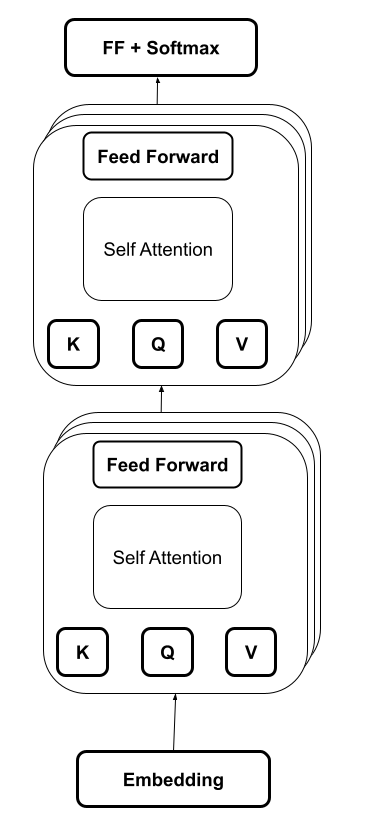
\includegraphics[scale=.35]{./images/transformerArchitectureSchematic.png}
\caption[Jeff Yoshimi with consultation from Tim Meyer.]{Schematic of the transformer architecture. Multiple blocks are stacked, capturing representational depth, as in a CNN. Each block contains a multi-head attention structure, where each head learns to represent inputs to the block in a different way. This captures representational width. The outputs of the multiple heads are combined in a standard feed-forward network. Other structures handling residual connections, and adding and norming activations, are not shown. As above, bolded items contain trainable parameters that are updated via gradient descent.}
\label{transformerArchitectureSchematic}
\end{figure}
 
Now we take a lesson from deep networks, and stack many of these transformer blocks on top of each other, to produce increasingly sophisticated representations. This is representational depth. Recall that with deep networks for vision, we get features, features of features, features of these features, etc. whose activations match neural response properties of different layers of the human visual system. This builds on the old idea of the \emph{Pandemonium} model (section \extref{cog_rev}), which involved (at successive layers): edge detectors, detectors for combinations of edges, detectors for combinations of these combinations (e.g. fragments of letters), and ultimately letter detectors. In a similar way, the successive layers of a transformer model of language correspond to increasingly complex features of the input stream, including syntactic categories, semantic properties, and far more complex features as well.\footnote{The extent to which activation patterns correspond to syntactic or semantic features is measured using post-hoc interpretation techniques such as probing. As with so many other neural network features, these were not ``programmed in'' by the engineers, but are emergent from the network after training, and are studied and described by scientists after the fact.}

The whole thing is trained using gradient descent and supervised learning (chapter \extref{ch_supervised}). It's the same ideas as with a simple feed-forward network trained using backprop, but with many more components trained. Items in bold in the figures above are trained: the word embedding, the key, query, and value matrices for each head in each block, and the normal weights and biases of the feed-forward networks. The error signals used in gradient descent are being back-propagated through a \emph{lot} of stuff here!

\subsection{Softmax Outputs}\label{llmOutput}

The first step in a transformer is to embed inputs, as we've seen. The next step is to transform these inputs using a series of blocks that are wide (thanks to multiple heads) and deep (thanks to multiple blocks). When all the processing is done, the last step is to un-embed the outputs, converting vectors back to tokens. 

In figure \ref{nextWordPrediction} we saw that while inputs use a word embedding, outputs are probability distributions over the whole vocabulary, and targets are one-hot encodings consisting of all zeros and a single ``hot'' number (the number 1) corresponding to the predicted next word (on one-hot encodings, see section \extref{wrangling}). When target data are binary one-hot encoded labels, the task given a network is a classification task (section \extref{classificationRegression}). Thus transformers are technically classifiers, which classify input texts according to what word is likely to occur next. Classification can here be seen as serving as a \emph{proxy task}. Our actual task is to predict a set of probabilities over next tokens. The output of an LLM is a set of probabilities over next tokens.\footnote{The interesting thing is that by \emph{trying} to perfectly classify next tokens (an impossible task), we end up with good probabilities, which is exactly we're after. Here is a way to think of it. If the model was trained to 100\% accuracy on the classification task, then it would always generate the same sentences from the same prompts (because it would assign one unique token to the current input). But then it could not generate new instances of text.}

The output of an LLM is often a \glossary{softmax} layer with around 50,000 outputs, which  indicate how probable all the tokens are given the input (all the prompts and responses in the context window so far). The softmax temperature parameter can be used here (see section \extref{wta_softmax_section}): higher temperatures will make the outputs more random or ``creative''. See figure \ref{transformerOverview} for how this might look for our simple example, where the output vocabulary just contains 7 tokens. 

%\begin{figure}[h]
%\centering
%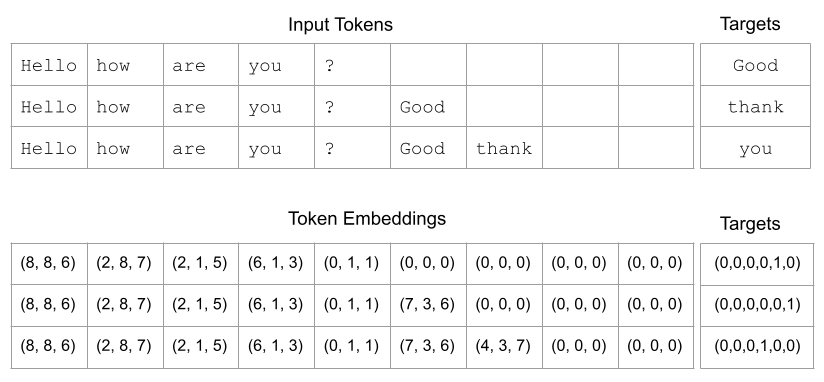
\includegraphics[scale=.45]{./images/contextWindow.png}
%\caption[Jeff Yoshimi]{What some training data might look like for the example in figure \ref{gptRecursedInputs}. The top panel shows the tokens in three training examples and the bottom row shows the corresponding token embeddings. The bottom panel shows inputs that can actually be fed into a neural network, in this case, a network with $9 \dot 4 = 36$ input nodes. Note that the targets are one-hot encoded, because these networks are actually classifiers (see section \ref{llmOutput}). Thus the output layer in this simple network would have 7 nodes for the 7 tokens: ``Hello'', ``how'', ``are'', ''you'', ``?'', "Good'', ``thank''. The softmax outputs are not shown, but for a well-trained network the outputs would be probability distributions close to the targets, for example $(0,0,.01,0,.99,0),  (.01,.01,0,0,0,.98), (0,.01,0,.98,0,.01)$. On softmax see section \extref{wta_softmax_section}}
%\label{contextWindow}
%\end{figure}

% Tim says it would be really nice to have this as a system diagram or like the multi head diagram above.
Once we have a probability distribution over tokens, we select one of the most probable next tokens and that becomes the output. This is usually done by sampling from among the top $n$ most probable next tokens. Thus the final softmax layer does the opposite of what the embedding layer does. Rather than converting from tokens to activations, it converts from activations to tokens, and is thus a ``de-embedding'' layer.

\subsection{Parameters and hyperparameters}

By way of summarizing, consider the parameters and  \glossary{hyperparameters} associated with a transformer-based LLM. Recall that parameters are primarily weights and biases (i.e values that are updated during training) while hyper-parameters are values that determine the structure of a network but that are not updated during training.

Figure \ref{gptParams} shows the  number of parameters for a range of GPT-3 subvarieties as $n_\text{params}$. The released version of GPT-3 had 175 billion weights and biases. By comparison, our xor 2-2-1 network had 3 biases and 6 weights, or 9 parameters. A standard convolutional neural network might have millions of parameters. So this is just massively larger. Not surprisingly, these networks have gotten even larger. GPT-4 has about 1.76 trillion parameters.\footnote{It takes large server banks that  consume huge amounts of energy to run these models, and so there is a thread of research attempting to achieve similar performance with smaller models, some of which can be run on a  personal computer. For example, Gemma2B achieves performance similar to GPT 3.5 with 2 billion parameter. See \url{https://developers.googleblog.com/en/smaller-safer-more-transparent-advancing-responsible-ai-with-gemma/}.} Figure \ref{gptParams} also shows the values of several hyperparameters such as number of layers ($n_\text{layers}$), corresponding to representational depth, and number of heads ($n_\text{heads}$), corresponding to representational width.\footnote{Notice that the size of the heads, $d_\text{head}$ is equal or almost equal to  $d_\text{model} \times n_\text{heads}$ (some mismatches are allowed).} The size of the token embedding  $d_\text{model}$ is also shown, as are the learning rate and batch size. Notice that these are all concepts we have seen in one way or another (often directly) in earlier chapters. All the same ideas are being used but on a larger scale.

\begin{figure}[h]
\centering
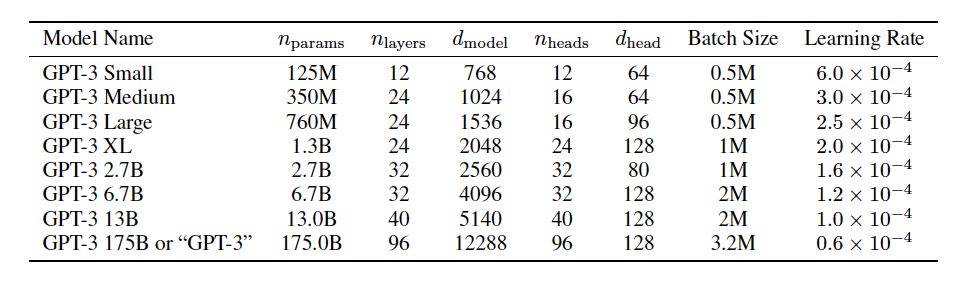
\includegraphics[scale=.4]{./images/gpt3_params.png}
\caption[\url{https://arxiv.org/abs/2005.14165}.]{Number of parameters and values for some of the hyperparameters used in training different versions of GPT-3. }
\label{gptParams}
\end{figure}

The size of the context window is another hyperparameter not shown in the figure. According to IBM research, ``when ChatGPT made its debut nearly two years ago, its window maxed out at 4,000 tokens. If your conversation went over the 3,000-word chat-interface limit, the chatbot was likely to hallucinate and veer off-topic. Today, the standard is 32,000 tokens, with the industry shifting to 128,000 tokens, which is about the length of a 250-page book. IBM just open-sourced on Hugging Face two Granite models with a 128,000-token window, and more are on their way.''\footnote{\url{https://research.ibm.com/blog/larger-context-window}.}

\section{LLMs in Practice}

This section discusses things you need to know to actually use an LLM in a functional system, like a tech stack (e.g. full stack development). It's one thing to know what an LLM is in terms of matrices etc.  But it is a totally separate thing to know how to integrate it with a meaningful piece of software, like having a person interface with it.  There are many practical matters to address.  For example should you fine tune it or not. All this stuff matters in a practical sense. 

Even though these are practical issues that have emerged around building effective LLMs, with virtually no thought to cognitive science, we've seen that historically it is not uncommon for engineering tools to end up being relevant. These ideas could be too, and they fill out more how LLMs work, so we include a discussion.  

Note: If you are reading this then you are reading an unpublished version of the text. Most of this section currently exists in latex comments.

% Pre-training vs. fine tuning. You have a pre-trained model and you take an additional special set of data and use that to slightly adjust the weights (e.g. with a lower learning rate). Lora fine-tuning involves a method where you take a subset of the weights and just fine-tune those. You find an optimal subset or add a set of weights and just adjust those for the task. A much lighter way to do fine tuning and better because you are not adjusting the whole model but in a sense just adding a ``bias-like'' term to your task. They find a kind of optimal smallest basis matrix, a bit like SVD (low rank adaptation). This is part of how deep seek did so well (as well as other things like good data cleanup; see that chapter). Fine tuning is updating an already existing LLM to bias it in favor of the language in some specified corpus you are interested in. For example you might download a llama 2 model, and then fine tune it based on a set of corpus using x library. See Kauf and Ivanova 2023. Video on fine tuning an LLM to talk about a set of PDFS (we can do it on all of Husserl): https://www.youtube.com/watch?v=dXxQ0LR-3Hg.  Or the Lou Reed example.  
% Lupyan notes, esp on what GPT3 was like and the role of fine tuning
% Video on fine tuning an LLM to talk about a set of PDFS (we can do it on Husserl): https://www.youtube.com/watch?v=dXxQ0LR-3Hg
% Pre-training on whole internet gets us background knowledge and solves the background knowledge problem (Dreyfus).  Or for BERT general linguistic competence. But fine-tuning makes it an expert in some domain.  Lora does not deeply teach it something new in all its weights, but rather shows how to do "one thing" in this bias like matrix.
% Reference back to Elman and staged learning.  Also the Cowan and activated long term working memory 
% Intuitive idea of things you know deeply in your bones from way back vs more recently learned
% Discuss fine-tuning vs pre-training and how ChatGPT-3.5, ChatGPT-4, etc. are fine-tuned variants of underlying GPT ``foundation models''.
% RLHF is Fine-tuning. But there are medical and legal ones too.  Use these examples it helps make it concrete. https://chatgpt.com/share/67e31bbf-9fe0-8007-bcb3-9804925e67ec
% Periodic updates to models should be covered. Also this is  way to contrasts prompts with fine tuning. When you ask about a current or recent event.

%  Prompt engineering.  This is the next step in adjusting your model. This determines the trajectory it takes in producing an input by changing the initial condition, the initial prompt. There is a light weight and heavy weight way to change how it runs (fine tuning). Then you can be more specific about what you are talking about.  Using your initial prompt and everyday language to corral how it produces an output. 
% Details. The user prompt gets put in a specific place in the template. Note idea of system vs. user prompt even if it is misleading. User prompt is just a special name for a part of the prompt template the use adds things to.  A job for cognitive scientists, not computer scientists (Tim). How do initialize LLMs so it provides outputs that are useful to people. Jail breaks.  System prompt contains instructions for the LLM not to do some things. In a jailbreak the user is figuring out what to add to the prompt template to override those instructions.   When you use it yourself and control the entire context window. This is happening ahead of time where you are given a role. Sometimes you can select these things, e.g on Azure.  We need a good picture (Tim has an example using langchain, which is pretty standard. Has "brackets" or "slots" that user input get stuck in). Maybe grab somethign form here: https://www.datacamp.com/tutorial/prompt-engineering-with-langchain
% Need to actually show an example system prompt (see leaked system prompts)
% myprompt template:
%	instructions: your instructions are ... 
%	my extra context {context}
%	examples: 
%		some examples here
%	user input: {userinputvar}
% Of course you could do this yourself as a user
% LLM orchestration is the overall script or code for how to feed in this or that value.  Cross-session memory is an example. Store some of this to be used again in a subsequent round.  
% Rags. Semantically encode a document. (ref to that chapter) Finds similar things from your corpus. Fills those semantically similar things into anther slot. So rather than filing up a giant context window, can selectively sample from it and the RAG will fill that. https://en.wikipedia.org/wiki/Retrieval-augmented_generation. Do a semantic encoding of your entire corpus. everything you want it to reference. Like a library of pdfs. Run a prelim system that goes through a datbase of pdfs and codes up each chunk in terms of what it's about. Then when you load your model it fits within a context window all the information that is as close as possible to your query. A way to fill the context window with relevant material when your overall corpus is too big to fit in the context menu. 
% Chain of thought reasoning is  a form of prompting where you get it to step through its reasoning process. As it explains how it's thinking it gives better answers by talking through its explanation.  Jeff has 3 orange, Tim eats 2, how many are left. Earlier models could struggle with this (find examples).  Even current models with novel models will just give you an answer and its not always as good. But better responses by doing this chain of thought thing.
% Basically it ranks context information from a larger store and decides what to add, because the context window itself has a limited size.
% Zero shot, one-shot, and few shot learning or prompting [note the comments here need to be checked; it appears that usage varies in different areas and that it sometimes does involve weight change].  Prompting better because our official def of learning in ch 1. is base don weight change, which this is not. Also called in-context learning.  These are all non-weight updates.  This can be thought of as prompt engineering, because it's stuff "learned" from how it deals with what you ask and what you put in the context window.  "learning" almost a misnomer. Weights are not updating. But can the model do something better based on what you give it in its context window.  You are changing its trajectory in activation space, not weight space.  Zero-shot uses no examples but just instructions. Example: zero thought chain of thought where you induce it by saying think it through. No examples, just better instructions. One shot means you give it an example. Think this through step by step, here's an example of what I mean.   You can do this yourself in your own prompts. A fancy name for something relatively simple.
% Reference back to old NN's not being able to do one-shot learning (and the use of that term in psychology).  Also working memory, and framing effects, and how the way you currently think of something separately from your existing conceptual apparatus can impact your behaviors.
% This is stuff you can get just from working memory, but it's never updating weights so that part is unrealistic.
% Prompt engineering as a job for cognitive scientists, not computer scientists (Tim). How do initialize LLMs so it provides outputs that are useful to people. 
% Multi-hop reasoning
% https://arxiv.org/abs/2403.09629 "Chain of Thought" it prompts itself


% Agentic systems [is that the right word? or agent, multi-agent]. Interfacing with other systems.  Consulting the net, executing python code.  The first layer is the LLM decides what jobs it needs to do. It then tells an agent to go do some jobs. Write a python script to do something then passes it off to another agent. Not sure how it’s related to internet searches or multihop reasoning.  Run a test, see if it works, and keep iterating until it works. Maybe cursor does this. Teams of LLMs or LLMs making calls to itself with different prompts. Example prompts to different people running a hospital. Send this prompt to nurse agent, send this to doctor agent. 
% Reference to cognitive models that involved different systems talking to each other.  Very plausible to think that LLMS describe something like how we answer questions or pull from unconscious memory, but they are clearly not capturing everything about humans. They have no self or goals or values or emotions (though they do capture how we _think_ about these things).
% See Millier part 2, 3.1.2. ‘Agent’ systems
% https://developers.googleblog.com/en/agent-development-kit-easy-to-build-multi-agent-applications/
% You can see this working in claude 2.7. Shows itself writing the code to call out to a console log what's in that document on the internet. LLM takes the task, breaks it up and sends bit of the task to different agents. LLM is instructed to take your task, decompose it, and pass those to different agents.
% Tim has a cool example of a simulated hospital: https://arxiv.org/html/2405.02957v3
% The relevance here is to the old cogsci debates of merging AI and Connectionism.
% They need not be separate LLMs. Just break down the task and have jobs. But can also be other kinds of agnets.

\section{Analysis of LLMs}\label{llm_analsis}

As with all the architectures discussed in this book, transformer-based LLMs are not just used to engineer useful devices, but are also major object of scientific interest (see chapter \extref{ch_applications}). They are studied in many academic disciplines and areas of cognitive science. They are being considered as models of cognition, linguistic processing, and neural processing. They are also being intensively scrutinized by the philosophical community.

% A difference in degree not kind. (A few points are mixed together here). It was not clear they would generalize so well. So a link to that. Can ask about situations etc. (See the dreyfus point). Pierre thought the best that would happen is grammar. (Jeff immediately tried old Dreyfus experiments and it passed). 
%These models have the remarkable property of being human engineered but not completely understood by the humans who engineered them. 
% Add some condensation of "LLMs being human-built but still of interest to science" below.

Here are some representative examples of recent research into LLMs. Here again, the landscape is rapidly changing, and this section will have to be frequently updated.

\subsection{LLMs and Cognitive Science}\label{llm_cogsci}

% This should be rewritten with stronger examples. Currently underwhelming in terms of what cognitive scientists have contributed historically and currently to LLMs. There is just this one brief discussion of the cog-sci benchmark.  Maybe consult Polyphony and Chris. 
% Also the bearing of all this on the debate with Chomsky is notably missing here. The sentence below, "That this was done by a neural networks has widely been seen as a decisive win for connectionism relative to the old debate about whether neural networks or symbolic architectures are best-suited to modeling cognition (see section \extref{cog_rev})." could go in some form here.

% I think we need to just make the basic point that insofar as they are realistic, they are realistic only about some _part_ of the mind. They don't have real emotion, or real goals or needs, or anxieties,  pragmatic concerns, or self, etc. It just corresponds to that part of us that "comes up with things to say" out of the depths of our souls.

A theme running through this book is that cognitive scientists are interested in neural networks, even when they originate in fields outside of cognitive science. That trend has continued with the emergence of large language models.

% Hard to get the import of this paragraph on a first read. Consider revising and maybe just making it shorter. 
% Cognitive scientists knew there were long-range dependencies in language. The old models failed at this.  See the supervised recurrent chapters. LLMs like BERT _could_ handle it. So LLMs are important to cogsci.
One obvious topic of interest to cognitive scientists is how transformers develop representations that are responsive to long-range dependencies in an input stream. A problem for earlier connectionist accounts of language processing was that they could not handle such dependencies. In an early paper on transformers co-authored by Jay McClelland  \cite{mcclelland2020placing} (a member of the original PDP group at UCSD; see section \extref{first_resurgence}), the following example is used to illustrate the point:
\begin{quote}
John put some beer in a cooler and went out with his friends to play volleyball. Soon after he left, someone \textbf{took the beer} out of the cooler. John and his friends were thirsty after the game, and went back to his place for some beers. When John opened the cooler, he discovered that the beer was \rule{1cm}{0.15mm}.
\end{quote}
What the reader expects in the blank spot depends on text earlier in the sentence. Here the reader expects the word ``gone'' next, but if ``took the beer'' is replaced with ``took the ice'' earlier in the sentence, the reader expects something like ``warm''. Transformers do quite well at this task. McClelland and colleagues describe transformers as using a ``query-based attention''  and have investigated the psychological and neural significance of the internal components of transformers when processing input streams. 

% Caucheteux et al. show that language model activations predict up to 40\% of brain activity during language processing \cite{caucheteux2022brains}. 
Recent work has gone much further with the project of understanding the psychological, computational and neural significance of transformers relative to human perception and cognition. Among current interests are papers that show that LLM representations are aligned with neural activations,  perceptual spaces, physical spaces and conceptual spaces. Abdou et al. show that language models can encode perceptual color relationships, even though they have never ``seen'' colors the way sighted humans have (but have only read about color relationship in texts) \cite{abdou2021can}. Liétard et al. find that LLMs can predict relative geographic distances between cities \cite{lietard2021do}. Christiansen et al. report that LLMs organize concepts in ways that correlate with human conceptual structures \cite{christiansen2023large}. These findings collectively suggest that LLM representations are not ``empty symbols'' as in traditional computer programs (see the discussion in \extref{classicalAIComparison}). Instead, they are content-rich and structured similarly to human mental representations.

Given these results, it seems likely that a lot of future research on LLMs will contribute to the field of cognitive science. Cognitive science also contributes to research on LLMs. For example, the LLM benchmark BIG-BENCH draws on cognitive science to test the ability to understand and combine concepts, including novel or invented concepts \cite{srivastava2022beyond}. Such benchmarks are not only used to assess LLM performance but also to refine and guide their development. 

\subsection{LLMs and Linguistics}

% Section a bit short. How have LLMs actually influenced linguistics research or theories. Say more about why linguistics researchers should care about this. How does this impact different approaches to linguistics: Chomskyan, Cognitive linguistics (Lakoff), etc.  Maybe ask Ryskin and Ellis.
Linguists have considered how these models handle syntax and semantics, revealing insights that bridge computational models and linguistic theory. For example, attention patterns in BERT and their correspondence to linguistic phenomena have been studied, and it has been shown that BERT's attention heads often focus on specific linguistic roles, such as the direct objects of verbs or the determiners of nouns \cite{clark2019does}. Interestingly, some attention heads display broad attention across entire sentences, while others are highly focused, suggesting a complex, multi-faceted approach to language understanding within the model. 

\subsection{LLMs and Neuroscience}

% More explanation needed here.

We have seen in earlier sections that neuroscientists have used convolutional neural networks (CNNs) to predict brain activity (section \extref{cnn_applications}). In a similar way, researchers are now leveraging transformer-LLMs to understand how our brains process language. 

% Discuss with Pierre whether to replace this discussion with a similar one using a more up-to-date reference
Schrimpf and colleagues \cite{schrimpf2021neural} explore how LLMs, like GPT and BERT, can predict neural responses during language comprehension. They proceeded by comparing brain activity of participants reading or listening to sentences with the activity patterns generated by these models. 

% Work and cohere with any material added on BERT. 
An interesting aspect of this study is the comparison between GPT and BERT. GPT, which processes language in a unidirectional manner (predicting the next word based on the previous words), was found to outperform BERT, which uses a bidirectional approach (considering the context from both directions). This suggests that our brain predicts unidirectionally, which  makes sense given that we usually are confronted with language orally and so get ``fed'' sentences word by word. 

% Removed given Eric S comments
%This provides some evidence for a theory of neuroscience called \emph{predictive processing}, which suggests that the brain is constantly making predictions about incoming sensory information to enable us to navigate the world.

\subsection{LLMs and Philosophy}\label{llmPhilosophy}

% Cite Chomsky's reaction to all this
% Eric S comments. Is this parrot argument a bit of a rehash of the Chomsky dismissal of statistical learning theory? Would Chomsky say they only confirm the poverty of the stimulus argument because they make use of billions times more data than actual humans? It might be nice to briefly discuss this. At any rate, it seems there are two arguments: one that statistical learning theory isn’t enough – that seems false. Two, poverty of the stimulus argument for human learning. That seems unclear as it likely depends on how you see the pretrained network humans are built with.  [Cohere this with discussion in the history chapter.]
% Integrate poverty of stimulus argument with stochastic parrot. Seems like the strongest counterarguent. Babies do it with way less data. Perhaps "inductive bias" is the way to fix it. Iris discussed it. 

Philosophers are also interested in LLMs given that they have arguably passed the Turing Test, and produced verbal behavior comparable to a human being. That this was done by a neural networks has widely been seen as a decisive win for connectionism relative to the old debate about whether neural networks or symbolic architectures are best-suited to modeling cognition (see section \extref{cog_rev}).  

But even if LLMs produce convincing behavior, do they really understand language? Doubts about the ability of machines to understand language have a long history, and there is a whole class of arguments to the effect that a system can’t understand the meanings of words just by manipulating meaningless symbols, or by transmitting meaningless information. These are sometimes called \emph{unusual realization arguments}, given that they
\begin{quote}
ask us to imagine people carrying out simple operations on bit streams, connectionist-like computations on activations patterns, or the control operations of the central processing unit of a computer. For example, Dneprov asks us to imagine a stadium full of people who pass 0’s and 1’s to one another on the basis of instructions announced over a loudspeaker. We can further imagine that this stadium is linked to an input-output device that enables it to pass the Turing test. We can then ask ourselves: do we really think this stadium full of people has consciousness or genuine understanding? \cite{noelle2022artificial}
\end{quote}

% ``an LM is a system for haphazardly stitching together sequences of linguistic forms it has observed in its vast training data, according to probabilistic information about how they combine, but without any reference to meaning: a stochastic parrot.''
% Clarify that this crituqes weak not strong AI
 One popular version of this argument as applied to LLM's is due to Emily Bender and colleagues \cite{bender2021dangers}, in which it is claimed that LLMs are ``stochastic parrots'' that capture nothing more than mere co-occurrence probabilities (in fact, the title of the paper includes a Parrot emoji). They formulate the problem using the thought experiment of an ``Octopus test'' \cite{bender2020climbing}, which goes like this: two English-speaking castaways communicate via telegraph across islands. A super-intelligent octopus intercepts their messages, learns the statistical patterns of the messages going back and forth, and, ``feeling lonely'', inserts itself into the conversation. Bender and Koller argue that the imaginary octopus could pass the test for simple chatbot-like interactions, but that it would fail in responding to strange situations involving words referring to objects the octopus has never perceived. This scenario is used to argue that, like the octopus, LLMs may produce seemingly meaningful outputs based solely on statistical patterns, without true understanding of language or the concepts they appear to discuss.

\begin{figure}[h]
\centering
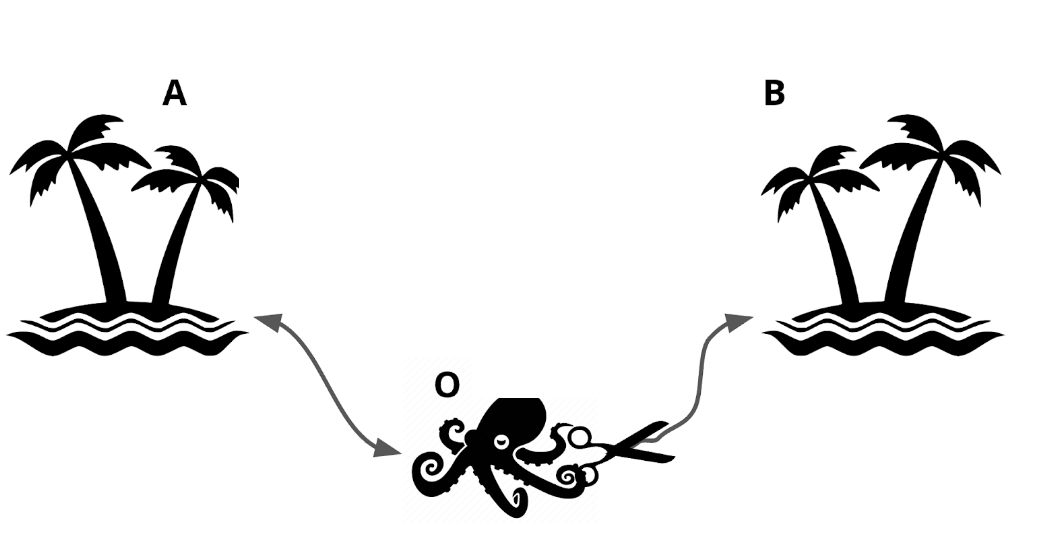
\includegraphics[scale=.20]{./images/octopusTest.png}
\caption[Soraya Boza.]{The octopus test. In the upper panel the octopus is observing the information being passed back and forth. At a certain point the octopus intercepts the wire and starts passing statistically similar messages to the person on the first island. This is shown in the lower panel. The communication is convincing, and the person on the left does not realize what has happened (the poor person on the right is just out of luck at this point). It has been argued that the octopus would not understand the information it passed along, even if it was convincing to the human. Moreover, it has been argued that the octopus would fail to produce convincing text in certain novel situations.}
\label{octopusTest}
\end{figure}

However, others argue that LLMs do understand the meaning of the words they produce. Relying on findings presented in section \ref{llm_cogsci}, Sogaard \cite{sogaard2023grounding} argues that the representations LLMs use are grounded (that is, are meaningful) in virtue of their alignment with human neural, cognitive, and perceptual spaces. These are not like the empty symbols passed along in Dneprov's stadium or in other ``unusual realization arguments.'' Here, the LLM (or the octopus) manipulates representations that have internal structures aligned with those of the human mind. In any case, the impressive results of models such as chatGPT fundamentally question not only empirical insights about language but also very deep philosophical conceptions about language.

Another long-standing argument against machine intelligence due to Hubert Dreyfus \cite{dreyfus1992computers} is that no computer or neural network could ever have truly human capacities, because they were not raised in the real world and can only parrot back what they were programmed or trained to say, at best with moderate abilities to generalize beyond that (Bender and Keller's argument develop this idea with respect to LLMs and argue these considerations are why the octopus would pass the test). However, humans with their embodied human existence develop an intuitive sense of the full context of the lived world. To show this, one of the authors (Yoshimi), who has regularly taught Dreyfus'  argument for many years, would have the class ask strange or unusual questions to AI systems and chatbots of earlier years, like ``What would happen if a penguin were to juggle alligators." The systems invariably struggled to say anything meaningful (though some chatbots did pretty well using tricks, like pretending to be a teenager saying ``lol who cares''). But chatGPT does just fine with the question, as you are welcome to see for yourself. Not everyone is convinced by this, and the discussion remains active. Melanie Mitchell, for example, has argued that these systems are not as intelligent as they appear, noting that there are many reasoning tasks they fail on \cite{mitchell2021ai}.

% https://www.researchgate.net/publication/380659127_Language_Models_Do_Not_Possess_the_Uniquely_Human_Cognitive_Ability_of_Relational_Abstraction
% Expand on Mitchell. She pulls out things that LLMs fundamentally can't do.  Feels a bit biased against LLMs passing the test.

% Discussion of LLMs being human-built but still of interest to science.

%There is something strange about LLMs. They were built by humans but are so complex that we do not completely understand them. This has often been the case historically with neural networks, but the issue is accentuated here. It's like we built this super powerful motor and now we can put it in different things, but we don't understand how the motor works so we have to look at its components and find new ways to study it, reverse engineer it, use it, etc. This may be a difference of degree (CNNs were also like this), but it is enough of a difference in degree that it feels like a change in kind.\footnote{One aspect of this is that with CNN's one could run a bunch on their own computer; with LLMs they are so expensive to train and it takes so long that people just make API calls to existing LLM models. So it feels more like this separately existing thing is just being studied, akin to studying any natural phenomenon in nature.} It really does feel different. These massive transformer-based neural networks with all their many layers and blocks and matrices and other features somehow magically produce human-like speech and video, etc., but how exactly is not understood. 
% 
%This is a twist on our earlier discussion of types of neural network research (chapter \extref{ch_applications}). It was built for engineering, but ended up being useful for science. Most earlier cases started in science and went to engineering (e.g. deep learning CNNs).
%
%The point was made striking early via BERT (which came out around the time of GPT-2). It came out of Google and fit their engineering needs. Psychologists and linguists then realized  BERT was doing better at analyzing language than other models in linguistics, so they started to treat it as an object of scientific interest in its own right. This gave rise to a new field called ``BERTology''. 
%
%As a result of this feature of LLMs, a huge ecosystem of analysis is growing up around them. Not all of it is obviously relevant to our focus here, cognitive science, but much of it is potentially relevant and it's too early to tell, so we here give a brief review.

%Engineers built something and then scientists created a science to understand it! In \cite{rogers2020primer} the authors explain:
%\begin{quote}
%Although it is clear that BERT works remarkably well, it is less clear why, which limits further hypothesis-driven improvement of the architecture. Unlike CNNs, the Transformers have little cognitive motivation, and the size of these models limits our ability to experiment with pre-training and perform ablation studies. This explains a large number of studies over the past year that attempted to understand the reasons behind BERT’s performance. In this paper, we provide an overview of what has been learned to date, highlighting the questions that are still unresolved.
%\end{quote}

% From https://www.pcgamer.com/software/ai/anthropic-has-developed-an-ai-brain-scanner-to-understand-how-llms-work-and-it-turns-out-the-reason-why-chatbots-are-terrible-at-simple-math-and-hallucinate-is-weirder-than-you-thought/: It's a peculiar truth that we don't understand how large language models (LLMs) actually work. We designed them. We built them. We trained them. But their inner workings are largely mysterious. Well, they were. That's less true now thanks to some new research by Anthropic that was inspired by brain-scanning techniques and helps to explain why chatbots hallucinate and are terrible with numbers.


